\documentclass[a4paper,11pt,listof=numbered,glossary=totoc,parskip=half,toc=bib]{scrreprt}
\usepackage[a4paper,left=2cm,right=2cm,top=2cm,bottom=2cm]{geometry}
\usepackage[onehalfspacing]{setspace}


\usepackage[colorlinks,
pdfpagelabels,
pdfstartview = FitH,
bookmarksopen = true,
bookmarksnumbered = true,
linkcolor = black,
plainpages = false,
hypertexnames = false,
citecolor = black]{hyperref}

\usepackage[utf8]{inputenc}
\usepackage[T1]{fontenc}
\usepackage[ngerman]{babel}
\usepackage{graphicx}
\usepackage{caption}
\usepackage[automake,toc,section=chapter,numberedsection]{glossaries}
\usepackage{uarial}
\usepackage{tabularx}
\usepackage{booktabs}
\usepackage{multirow}
\usepackage{icomma} % Damit im Mathemodus nach einem Komma kein Leerzeichen gesetzt wird
\usepackage[cache=false]{minted}
\renewcommand{\listoflistingscaption}{Verzeichnis der Code-Listings}
\usepackage[table]{xcolor} % Zum Ändern der Farben in Tabellen

\usepackage{csquotes}
\usepackage[backend=biber, style=apa]{biblatex}
\addbibresource{quellen.bib}

\renewcommand{\familydefault}{\sfdefault}

\RedeclareSectionCommand[
beforeskip = 3pt,
afterskip = 3pt]{subsection} %vor subsection 6pt und nach subsection 6pt Abstand
\RedeclareSectionCommand[
beforeskip = 1pt,
afterskip = 1pt]{subsubsection} %vor subsection 6pt und nach subsection 6pt Abstand


% Glossar
\makeglossary
\newglossaryentry{re}
{
	name={Requirements Engineering (RE)},
	description={Das \textit{Requirements Engineering} bezeichnet die Disziplin der Anforderungsermittlung. Damit ist typischerweise das Ermitteln, Dokumentieren, Prüfen und Abstimmen von funktionalen und nicht-funktionalen Anforderungen gemeint.}
}

\newglossaryentry{stakeholder}
{
	name={Stakeholder},
	description={\textit{Stakeholder} (dt. Anspruchsgruppen) sind alle Personen, die mit dem zu entwickelnden System konfrontiert sind.
Der Begriff beschränkt sich nicht nur auf diejenigen, die unmittelbar mit dem System arbeiten, sondern schließt insbesondere den Auftraggeber, das Entwicklerteam oder die mit dem Betrieb des Systems betrauten Personen mit ein.}
}
\newglossaryentry{userstory}
{
	name={User Story},
	description={Eine \textit{User Story} ist eine besonders in agilen Projekten weit verbreitete Dokumentationsform im Kontext der Anforderungsermittlung.
Sie besteht aus einem einfachen Satz, der eine Anforderung aus der Sicht einer definierten Stakeholder-Rolle beschreibt und entspricht immer einem fest vorgegebenen Format:
\textit{Als [Rolle] möchte ich / wünsche ich mir [Funktion], damit [Begründung].}
User Stories lassen sich damit auf einfache Karteikarten schreiben, die an ein Whiteboard gepinnt oder auf einem großen Tisch ausgebreitet werden können. Somit lassen sie sich gut in Workshops zur Visualisierung und Priorisierung der Anforderungen nutzen.}
}
\newglossaryentry{moscow}
{
	name={MoSCoW},
	description={Die \textit{MoSCoW-Methode} wird im vorliegenden Projekt genutzt, um Anforderungen zu priorisieren.
\textit{Must have (M)} legt fest, dass die betrachtete Anforderung zwingend umgesetzt werden muss.
\textit{Should have (S)} bedeutet, dass die Umsetzung wünschenswert, aber nicht kritisch ist.
\textit{Can have (C)} bezeichnet unkritische Anforderungen, die optional zu einem späteren Zeitpunkt implementiert werden können.
\textit{Won't have (W)} legt fest, dass die betrachtete Anforderung (aktuell) nicht umgesetzt wird.
Die Priorisierung von Anforderungen ist nicht endgültig, sondern kann im Projektverlauf angepasst werden.
	}
}
\newglossaryentry{git} 
{
	name={Git-Repository},
	description={GIT ist ein Werkzeug zur Versionskontrolle, dass vor allem zur kollaborativen Quellcode-Verwaltung in Software-Projekten eingesetzt wird, sich aber auch zur Verwaltung und Versionierung von Artefakten der Dokumentation eignet.
Die von Microsoft betriebene Plattform GitHub.com bietet einen Dienst für das Hosting von Git-Repositories.}
}
\newglossaryentry{responsive}
{
	name={Responsive Design},
	description={Ist eine Applikation so gestaltet, dass sie sich an verschiedene Bildschirmgrößen und -ausrichtungen, wie sie beispielsweise bei Smartphones-, Tablets oder Desktop-PCs zu finden sind, anpassen kann, so spricht man von \textit{Responsive Design}.
	}
}
\newglossaryentry{uml}
{
	name={UML},
	description={Die \textit{Unified Modeling Language} ist eine grafische Modellierungssprache zur Analyse, Implementation und zum Design von softwarebasierten Systemen sowie zur Beschreibung von Prozessen. \autocite{UML} Sie wird durch die \textit{Object Management Group} entwickelt. Die Sprache definiert jeweils sieben Struktur- und Verhaltensdiagramme.
	In diesem Bericht werden folgende Diagrammtypen genannt:
	\begin{itemize}
	\item cod:	Komponentendiagramm
	\item cld:	Klassendiagramm
	\item sm:	Zustandsdiagramm
	\item sqd:	Sequenzdiagramm
	\end{itemize}
	}
}
\newglossaryentry{bpmn}
{
	name={BPMN},
	description={Die \textit{Business Process Model and Notation} ist ein Standard zur grafischen Spezifikation von Geschäftsprozessen. \autocite{BPMN} 
	}
}
\newglossaryentry{erm}
{
	name={ERM},
	description={Ein \textit{Entity-Relationship-Model} ist ein Modell zur Darstellung von Entitäten und Beziehungen. Der Einsatz von ERM gilt als Standard bei der Datenmodellierung in der Softwareentwicklung.
	}
}
\newglossaryentry{gui}
{
	name={GUI},
	description={Grafische Benutzeroberfläche
	}
}

\subject{Meilensteinbericht}
\title{Meilenstein 3}
\subtitle{Dokumentationskonzept bereitgestellt}

\begin{document}
	\pagenumbering{Roman}
	\begin{titlepage}
		
		\centering
		\vspace*{2.5cm}
		{\large\bfseries Meilensteinbericht\par}	
		{\Huge\bfseries Meilenstein 3\par}
		{\Large\bfseries Dokumentationskonzept bereitgestellt\par}

		{\Large Projekt Q-Teams\par}
		{\large\today\par}
		\vspace{0.5cm}

			
		
		
\includegraphics[scale=0.5]{iubh_logo}
		
		IUBH Fernstudium
		\vspace{0.5cm}
		
		\begin{tabular}{lllrl}
			\toprule
			\textbf{Gruppe} & \textbf{Nachname} & \textbf{Vorname} & \textbf{Matrikelnr.} & \textbf{Studiengang} \\
			\midrule
			Projektleiter & Sawatzki & Jörg & 9186524 & BSc. Informatik \\
			Mitglied 2 & Hahn & Maximilian & 91710055 & BSc. Wirtschaftsinformatik \\
			Mitglied 3 & Lapenat & Holger & 3191237 & BSc. Wirtschaftsinformatik \\
			Mitglied 4 & Moch & Daniel & 91710824 & BSc. Wirtschaftsinformatik \\
			\bottomrule
		\end{tabular}	
	\end{titlepage}
	
	
	\newpage
	\setcounter{tocdepth}{1}
	\tableofcontents
	
	\newpage
	\pagenumbering{arabic}	
	\chapter{Beschreibung der Projektdokumente}

	Im Verlauf des Projektes werden verschiedene Dokumente erstellt und gepflegt. Diese unterstützen das Projektmanagement oder informieren Stakeholder über den Status bestimmter Aspekte des Projekts.
	
	Der Aufbau des Risikoregisters ist bereits im Bericht zum Meilenstein 1 definiert worden. Die weiteren Dokumente werden im Folgenden definiert.
	
	\section{Aufgabenliste}
	Die Gesamtheit der Aufgaben, die durch das Team zu erledigen sind, werden in der Aufgabenliste geführt. Alle Aufgaben werden als Ticket im System Redmine geführt. Die zu pflegenden Informationen jedes Tickets sind in Tabelle \ref{tab:tickets} dargestellt. 
	
	Für die Implementierung werden nur die User Stories als Tickets angelegt, die bereits im Bericht zum Meilenstein 1 vorgestellt wurden (\cite{MS1}, S. 5f). Die weitere Verfeinerung der User Stories und die Ableitung der Aufgaben findet im GitHub Issue Tracker statt. Das heißt, dass die Implementierung nur sehr grob in Redmine abgebildet ist. Dieser Schnitt wird vollzogen, um den direkten Bezug der Implementierungsaufgaben zum Quellcode herstellen zu können. Da auch die Anzahl der in Redmine anfallenden Tickets deutlich reduziert wird, hilft dieses Vorgehen außerdem dabei, den Gesamtüberblick über das Projekt nicht zu verlieren.
	\begin{table}
		\centering
		\begin{tabularx}{\textwidth}{lX}
			\toprule
			\textbf{Aspekt} & \textbf{Beschreibung} \\
			\midrule
			Titel & Aussagekräftige Bezeichnung des Tickets \\
			ID & Für das Projekt eindeutige Identifikationsnummer \\
			Status & New / In Progress / Feedback / Closed \\
			Priorität & Low / Normal / High / Urgent \\
			Zugewiesen an & Die Person, die für die Bearbeitung des Tickets verantwortlich ist \\
			Übergeordnete Aufgabe & Jedes Ticket kann einem anderen Ticket untergeordnet werden. Hier wird das dann übergeordnete Ticket angegeben. \\
			Beginn und Abgabedatum & Falls erforderlich kann ein Beginn und Ende der Bearbeitung angegeben werden. \\
			Beschreibung & Hier wird das erforderliche Ergebnis beschrieben.\\
			\bottomrule
		\end{tabularx}
		\caption{Aufbau von Tickets im Redmine-System}
		\label{tab:tickets}
	\end{table}	
	
	\section{Sprint Backlog}
	Die Tickets, die im folgenden Sprint bearbeitet werden sollen, werden mit \textit{High} oder \textit{Urgent} priorisiert. Um ein Ticket als besonders dringend zu kennzeichnen, kann die höhere der beiden Priorisierungen genutzt werden, grundsätzlich wird hier jedoch die Priorität \textit{High} genutzt. Die Menge dieser Tickets bildet den Sprint Backlog, ein seperates Dokument wird nicht gepflegt. Der Lebenszyklus eines Tickets wird in Abbildung \ref{fig:ticketlebenszyklus} dargestellt. Während der Sprintplanung und während des Sprints werden die Tickets des Sprint Backlogs an die Teammitglieder zur Bearbeitung zugewiesen. Nach der Bearbeitung wird dem Team ein Ergebnisentwurf zur Verfügung gestellt wird. Das Team führt nun die festgelegten Qualitätssicherungsmaßnahmen durch, falls diese nicht bereits Bestandteil des vorherigen Bearbeitungsprozesses waren. Das Ergebnis wird anschließend freigegeben oder es werden Änderungen eingearbeitet. Die fertig bearbeiteten Tickets werden nicht gelöscht, sondern verbleiben als geschlossene Tickets in der Anforderungsliste.
	\begin{figure}
		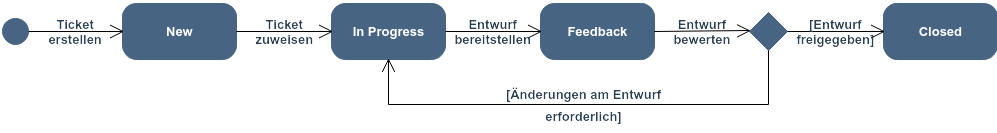
\includegraphics[width=\textwidth]{Ticketlebenszyklus}
		\caption{Lebenszyklus eines Tickets}
		\label{fig:ticketlebenszyklus}
	\end{figure}
	
	
	\section{Ergebnisdokumentation}
	Das ausgelieferte Softwareprodukt wird in der Ergebnisdokumentation beschrieben. Nachfolgend werden die einzelnen Aspekte dieser Dokumentation vorgestellt.
	
	\subsection{Funktionsbeschreibung}
	Der in der Anwendung umgesetzte Geschäftsprozess wird aus der Sicht eines Nutzers mit der \Gls{bpmn} dargestellt. Es werden die unterstützten Fachfunktionen benannt und in den Gesamtkontext gebracht. Die wichtigsten Fachfunktionen werden detailliert beschrieben.
			
	\subsection{Softwarearchitektur}
	\label{subsec:softwarearchitektur}
	Die Softwarearchitektur wird aus verschiedenen Sichten beschrieben, in Tabelle \ref{tab:softwarearchitektur} sind diese dargestellt. Außerdem werden die zur Visualisierung zu nutzenden Modelle festgelegt.
	
	\begin{table}
		\centering
		\begin{tabularx}{\textwidth}{lXl}
			\toprule
			\textbf{Sicht} & \textbf{Beschreibung} & \textbf{Modell} \\
			\midrule
			Systemstruktur & Die Komponenten und die Schnittstellen der Anwendung werden in einem Überblick dargestellt. & \Gls{uml}-cod \\
			Daten & Das technische Datenmodell mit den Entitätstypen, den zugehörigen Attributen und den Beziehungen untereinander wird dargestellt.  & \Gls{uml}-cld \\
			\Gls{gui} & Die in der grafischen Benutzeroberfläche möglichen Zustände und die erlaubten Übergänge zwischen diesen werden dargestellt. Die visuelle Gestaltung der GUI (z.B. in Form von Screenshots) wird hier nicht dargestellt. & \Gls{uml}-sm\\
			Komponenten & Bei Bedarf werden einzelne Komponenten des Systems detaillierter dargestellt. & \Gls{uml}-cod \\
			Zeit & Bei Bedarf werden einzelne Aufrufbeziehungen zwischen Komponenten detailliert dargestellt. & \Gls{uml}-sqd \\
			\bottomrule
		\end{tabularx}
		\caption{Sichten und genutzte Modelle für die Dokumentation der Softwarearchitektur}
		\label{tab:softwarearchitektur}
	\end{table}	
	
	
	\subsection{Anhang}
	Tabelle \ref{tab:ergebnisdokumentation_anhang} stellt dar, welche weiteren Aspekte im Anhang aufgelistet werden.
	\begin{table}
		\centering
		\begin{tabularx}{\textwidth}{lX}
			\toprule
			\textbf{Aspekt} & \textbf{Beschreibung} \\
			\midrule
			Anforderungen & Die während des Projektzeitraums umgesetzten Anforderungen werden dargestellt. Zu jeder Anforderung wird der Erfüllungsgrad der Akzeptanzkriterien dargelegt. Nicht umgesetzte Anforderungen werden aufgelistet. \\
			Qualitätsziele & Die Erfüllung der Qualitätsziele und die durchgeführten Maßnahmen zur Qualitätssicherung werden zusammenfassend dargestellt. \\
			Benutzerhandbuch & Der Benutzer wird über die bestimmungsgemäße Nutzung der Anwendung informiert. Das Benutzerhandbuch wird in deutscher Sprache verfasst sein. \\
			Administration & Die Tätigkeiten zur Administration der Anwendung werden in einem Handbuch beschrieben. \\
			Inbetriebnahme & Die erforderlichen Schritte zur Installation und Inbetriebnahme auf einem anderen System werden beschrieben. \\
			\bottomrule
		\end{tabularx}
		\caption{Anhang der Ergebnisdokumentation}
		\label{tab:ergebnisdokumentation_anhang}
	\end{table}
	
	\section{Projektdokumentation}
	Eine Projektdokumentation informiert abschließend über den gesamten Verlauf des Projektes. Da zu diesem Projekt ein abschließender Projektbericht erstellt wird, beschränkt sich die hier zu erstellende Projektdokumentation auf die Darstellung des Entwicklungsfortschritts auf der Zeitachse. Dazu werden jeweils die Ergebnisse der Sprints zusammengefasst. Die Projektdokumentation soll dem Auftraggeber dazu dienen, die Arbeitsleistung des Projektteams ex post bewerten zu können.
	 
	\section{Testprotokoll} % kommt von Holger?! 
	
	\section{Risiko-Wert-Matrix}
	\label{sec:risikowertmatrix} % Ist mir auch irgendwie nicht Projektspezifisch genug. Könnte man also ggf. weglassen.
	Die Bearbeitungsreihenfolge von Aufgaben im Projekt kann nicht willkürlich festgelegt werden. Einschränkend gibt es in nahezu jedem Fall Abhängigkeitsbeziehungen zwischen den Aufgaben. Auch andere Rahmenbedingungen können die Freiheitsgrade weiter einschränken. Die dann noch erforderliche Reihung der Aufgaben wird durch die Risiko-Wert-Matrix in Abbildung \ref{fig:risikowertmatrix} unterstützt. Mit Hilfe dieser Matrix wird zum Einen das \textit{Fail-Fast-Prinzip} umgesetzt. Demnach sollten Risiken möglichst frühzeitig angegangen werden. Ein Scheitern (engl. \textit{fail}) sollte somit möglichst zu einem frühen Zeitpunkt passieren, eben schnell (engl. \textit{fast}). Zum Anderen wird der Fokus auf wertbringende Aufgaben gelegt. Unter Berücksichtigung der Faktoren Risiko und Wert ergibt sich somit eine Umsetzungsreihenfolge.
	
	\begin{figure}
	\centering
	\renewcommand{\arraystretch}{2}	
	\begin{tabular}{rrccc}	
		\arrayrulecolor{white}
		& & &  \multicolumn{2}{c}{\textbf{Umsetzungsreihenfolge}} \\ 
		\multirow{2}{*}{\rotatebox{90}{\textbf{Risiko}}} &
		\cellcolor[HTML]{bee3d3}Hoch  && \cellcolor[HTML]{F6D8CE} Vermeiden & \cellcolor[HTML]{D8F6CE} Als Erstes umsetzen\\
		&\cellcolor[HTML]{bee3d3}Niedrig && \cellcolor[HTML]{F5ECCE}Zuletzt umsetzen & \cellcolor[HTML]{ECF6CE}Als Zweites umsetzen \\ \cmidrule[6pt]{3-4}
		&&& \cellcolor[HTML]{c2e0ae}Niedrig & \cellcolor[HTML]{c2e0ae}Hoch\\ 
		&&& \multicolumn{2}{c}	{\textbf{Wert}}
	\end{tabular}
	\caption{Risiko-Wert-Matrix}
	\label{fig:risikowertmatrix}
\end{figure}

	\newpage
	\chapter{Implementierung}
	% @toDo einleitende Worte	
	
	\section{Implementierungsprozess}
	Wie der gesamte Softwareentwicklungsprozess wird auch die Implementierung agil durchgeführt. Die Definition der Rahmenbedingungen wurde bereits im Bericht zum Meilenstein 1 dargelegt (\cite{MS1}, S.12ff). 
	
	Im ersten Schritt der Implementierung wird die Grobstruktur des Systems erarbeitet. Die Reihenfolge der zu erstellenden Softwareartefakte ergibt sich einerseits durch die strukturellen Abhängigkeitsbeziehungen. Damit ist z.B. die Abhängigkeit des Backends von den im Frontend gewonnen Daten gemeint.\footnote{Auf die Erstellung von Dummies oder Treibern wird in diesem Projekt verzichtet.} Andererseits ergeben sich durch den fachlichen Prozess zeitliche Abhängigkeiten. Dem bezüglich der Implementierungsreihenfolge übrigen Entscheidungsspielraum wird mit der Risiko-Wert-Matrix (siehe Abschnitt \ref{sec:risikowertmatrix}) begegnet.
	
	\section{Rollenverteilung}
	Die Rollenverteilung während der Implementierung ergibt sich ebenfalls aus den Festlegungen, die im Bericht zum Meilenstein 1 getroffen wurden. Diese Zuordnung ist allerdings nicht trennscharf, denn zwischen den Themenbereichen gibt es Überschneidungen und Verknüpfungen. Nach Themenbereich geordnet ergibt sich folgende Verteilung:
	
	\subsubsection{Backend-Entwicklung}
	Jörg Sawatzki, Maximilian Hahn
	
	\subsubsection{Frontend-Entwicklung}
	Jörg Sawatzki, Daniel Moch
	
	\subsubsection{Qualitätssicherung}
	Holger Lapenat

	\newpage
	\chapter{Qualitätsmanagement}
	
	
	\printglossaries
	\newpage	
	\printbibliography[heading=bibnumbered,title=Literaturverzeichnis]

\end{document}
